

\documentclass[aspectratio=169, 12pt]{beamer}

%%%%%%%%%%%%
% Packages %
%%%%%%%%%%%%

\usepackage{ctex}
\usepackage[english]{babel}
\usepackage{packages/sleek}
\usepackage{packages/tweaks}
\usepackage{calligra} % thanks pakeage
\usepackage{graphicx}

%%%%%%%%%%%%%%%%
% Bibliography %
%%%%%%%%%%%%%%%%

\addbibresource{./resources/bib/references.bib}

%%%%%%%%%%%%%%
% Title-page %
%%%%%%%%%%%%%%


\title{公共经济学}
\subtitle{Public Economics}
\author[LIU ShHUAI]{刘 {  } 帅}
\institute{山西师范大学 {  } 经济与管理学院}
\date{\today}
\titlelogo{./resources/pdf/logo.png}
\framelogo{./resources/pdf/logo.png}

%%%%%%%%%%%%
% Document %
%%%%%%%%%%%%

\begin{document}

\maketitle

\begin{frame}[standout]
    第五章\par
    \addtolength{\parskip}{.4em}
    市场失灵
\end{frame}

\begin{frame}[plain]
    \frametitle{重点问题}
    \begin{itemize}
        \item \textbf{市场不能产生有效结果的主要原因是什么?}
        \item \textbf{政府在使市场顺利运转过程中起什么作用?}
        \item \textbf{如果市场的资源配置具有帕累托效率,为什么政府还要进行干预?什么是有益产品?政府在再分配中的作用是什么?}
        \item \textbf{什么是政府作用的“市场失灵”说?思考政府作用的其他视角包括哪些?}
    \end{itemize}
\end{frame}

\begin{frame}[plain]
    % \begin{multicols}{1}
    %   \frametitle{Outline}
    %   \tableofcontents[hideallsubsections]
    % \end{multicols}
    \frametitle{Outline}
    \tableofcontents[hideallsubsections]
    % \tableofcontents[currentsection]
\end{frame}

\section{一、产权与合同履行}

\begin{frame}[plain]
    \frametitle{产权与合同履行}
    市场要发挥作用,需要政府界定产权和强制履行合同。
    当土地是共有财产时,任何人都可以在土地上放牧。
    由于没有人拥有土地的产权,也就没有人有动力保证不过度放牧,这一现象称之为公地悲剧。
    \par
    同样的,如果人们彼此间进行交易,所签订的合同就必须执行。
    就拿一笔典型的贷款来说,一个人向别人借钱,签署了一份偿还合同。
    如果这份合同得不到履行,肯定没有人愿意把钱借出去。
    \par
    从更简单的角度来讲,如果没有对私人财产的保护,人们就不会有足够的储蓄和动机,
    因为他们的储蓄可能被剥夺。
    \par
    旨在保护公民生命及财产强制履行合同和界定产权的政府活动,可以被视为所有市场经济赖以存在的基础。
\end{frame}

\begin{frame}[plain]
    \frametitle{产权与市场失灵:重新审视公地悲剧}
    公地悲剧中最常说的例子是公共草场因过度放牧而遭破坏,
    或公共湖泊因过度捕捞而枯竭。虽然每个人的行为都是理性的,
    都想增加自身的短期私利,但整个群体的集体行为不符合社会长期最佳利益。
    \par
    如何管理一种没有明文规定属于任何人的资源?
    \par
    长期以来,一般的解决办法是,或将公共资源转化为私有财产,或对这些
    公共资源进行外部监管。如果某种资源被转变为私有财产,其所有者
    应该有利润动机并进行产权保护,负责任地管理这种资源。如果资源由政府监管,
    要从公共利益出发对个人用户约法三章。
\end{frame}

\begin{frame}[plain]
    \frametitle{产权与市场失灵:重新审视公地悲剧}
    然而,2009年诺贝尔经济学奖获得者埃利诺$\cdot $奥斯特罗姆重新
    审视了这些方案。以前属于公共的资源被私人控制可能引发垄断行为,而外部监管
    可能会引发不适当的、难以执行的法律法规。通过经验总结,她提出解决
    公地悲剧的第三种方案:利用社区的社会资本设计出富有创造性和有效性的本地解决方案。
    \par
    在这场辩论中,出现另一个术语——反公地悲剧,这是哥伦比亚大学法学院迈克尔$\cdot $海勒的自造词。
    反公地悲剧指的是相反的情形:社区资源的过度私人化,从社会角度来看达不到理想的结果。
    现在反公地悲剧普遍应用于类似生物医学研究领域的过度产权,比如基因的专利申请。
\end{frame}

\section{二、市场失灵与政府作用}

\begin{frame}[plain]
    福利经济学第一定理认为,只有在特定的环境和条件下,经济才会达到帕累托效率。
    在6种重要情况下,市场无法实现帕累托效率,称为市场失灵,这为政府活动提供了理论依据。
\end{frame}

\begin{frame}[plain]
    \frametitle{不完全竞争}
    导致帕累托效率的市场一定是完全竞争的,即必须有足够多的企业,
    每个企业都认为他不影响价格。
    \par
    然而,在某些行业,比如超级计算机、电脑操作系统和芯片、铝、烟草、
    等行业,企业相对较少,或者其中的一两家企业占据了市场的较大份额。
    只存在一家企业供应市场时,经济学家称这种形式为\textbf{垄断(monopoly)};
    有几家企业供应市场时,经济学家称这种形式为\textbf{寡头垄断(oligopoly)}。
    即使有许多家企业,每家企业也可能生产稍有差别的产品,因而可能会认为自己面临
    向下倾斜的需求曲线。经济学家称这种情形为\textbf{垄断竞争(monopoly competition)}。
    以上所有这些情形都偏离了理想的完全竞争(每个企业都如此小,以至于认为自己不可能影响价格)。
\end{frame}

\begin{frame}[plain]
    \frametitle{不完全竞争}
    \begin{figure}
        \centering
        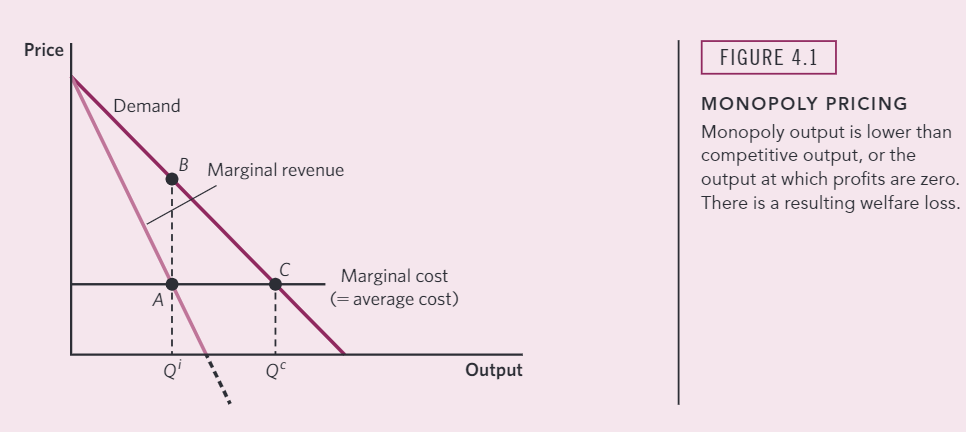
\includegraphics[width=1.0\textwidth]{./resources/figure/monopoly.png}
    \end{figure}
\end{frame}

\begin{frame}[plain]
    \frametitle{公共产品}
    有些产品,市场不提供,或者即使提供,数量也不足。规模大的例子如国防;
    规模小的如导航设施(如浮标)。这些都被称为纯公共产品。
    纯公共产品有两个关键属性:
    \begin{block}{非竞争性}
        多一个人受益不会增加任何成本:正规的说,多一个人享用这种产品
        的边际成本为零。保卫一个人口101万人的国家的成本不会比保卫一个100
        万的国家高;灯塔的成本与经过的船只数量无关。
    \end{block}
    \begin{block}{非排他性}
        一般而言,难以或不可能把某些人排除在享用纯公共产品之外。
        假如我为了自己航行安全在礁石丛生的航道上建了一座灯塔,我很难
        或不可能将通过航道并享受航行好处的船只排除在外。如果我们的
        国防政策成功抵御了外侵,那么每个人都受益,没有办法让某个人不享有这些好处。
    \end{block}
\end{frame}

\begin{frame}[plain]
    \frametitle{外部性}
    在许多情况下,一个人或一家企业的行为会影响其他人或其他企业,比如,
    一家企业给其他企业造成成本而没有予以补偿,或者一家企业给其他企业带来
    利益而没有获得相应的报酬。空气污染和水污染就是其中的例子。当我开的车没有减排
    装置时,我降低了空气质量,让其他人付出了代价。同样地,一家化工厂
    将化学物质排入附近的河流,给下游河水的用户造成了损失,因为后者要使用河水
    就得花大笔资金净化河水。这些都是外部性的例子。
\end{frame}

\begin{frame}[plain]
    \frametitle{外部性}
    \textbf{负外部性}是指一个人的行为给其他人带来成本的情形,不过,
    并非所有的外部性都是负的,有些重要的情形属于\textbf{正外部性}——一个人的行为给他人带来了好处。
    \par
    只要存在这些外部性,市场配置资源就不会是有效率的。
    由于个人不承担他们自己所产生的负外部性的全部成本,他们从事
    的这类活动就会过多;相反,由于个人不享有正外部性活动的全部利益,他们从事的这类活动就会过少。
\end{frame}

\begin{frame}[plain]
    \frametitle{不完全市场}
    纯公共产品和服务并不是私人市场不能充分提供的唯一产品和服务。
    只要私人市场不能提供产品和服务,即使提供的成本低于个人的支付意愿,市场失灵就存在,
    我们称这种情形为\textbf{不完全市场}。\par
    一些经济学家认为,私人市场在提供保险和贷款上的表现特别糟糕。
    在过去40年里,为什么资本市场和保险市场是不完全的,一直是广泛研究的主题。
    关于不完全资本和保险市场的解释至少有三种,每一种都有一定的道理。
    \par
    第一种解释强调创新,认为新证券和新保单自我创新不足。
    \par
    第二种解释强调交易成本,市场运作、履行合同和新产品的推广,代价高昂。
    \par
    第三种解释强调信息不对称和实施成本较高,道德风险,逆向选择。
    \par
    互补市场缺失也是造成不完全市场的原因之一。
\end{frame}

\begin{frame}[plain]
    \frametitle{不完全市场}
    不完全市场的原因对政府如何弥补市场失灵可能有所启发。
    不过,政府也要面对交易成本、实施问题和信息不对称,
    尽管许多情况下与私人部门所面对的问题不同。因此,在设计贷款项目
    或干预资本市场时,政府也需要牢记:自己知道的往往没有借款人知道的多。
\end{frame}

\begin{frame}[plain]
    \frametitle{不完全信息}
    所谓不完全信息(Incomplete Information)是指市场参与者不拥有某种经济环境状态的全部知识。
    \par
    信息不完全不仅是指那种绝对意义上的不完全,即由于认识能力的限制,人们不可能知道在任何时候、任何地方发生任何情况,而且是指“相对”意义上的不完全,即市场经济本身不能够生产出足够的信息并有效的配置它们。
    \par
    在现实经济中,信息的传播和接受都需要花费成本,而市场通信系统的局限和市场参与者释放市场噪声等客观和主观因素的影响也都将严重阻碍市场信息的交流和有效的传播。结果,价格信息不可能及时传递给每一个需要信息的市场参与者,而每个市场参与者所进行的交易活动及其结果也不可能及时地通过价格体系得到传递,因而市场价格不可能灵敏地反映市场的供求状况,市场供求状况也不可能灵敏地随着价格的指导而发生变化,市场机制可能因此失灵。
\end{frame}

\begin{frame}[plain]
    \frametitle{失业、通货膨胀与失衡}
    大多数经济学家都把高失业率视为市场在有些事情上没有做好的
    初步证据。在有些经济学家看来,高失业率是最为引人注目的、最具有
    说服力的市场失灵的证据。
\end{frame}

\begin{frame}[plain]
    \frametitle{各种市场失灵之间的关系}
    我们所讨论的市场失灵并不是相互排斥的,信息问题常常部分地解释了
    市场缺失问题,而外部性经常被认为是由市场缺失所致:
    如果能对使用渔场的渔民收费——存在捕鱼权市场,就不会出现过度捕捞。
    有时,公共产品被视为外部性的极端情况——其他人从我的公共产品生产种受益,我也从
    其他人的公共产品生产中受益。
\end{frame}

\section{三、再分配与有益产品}

\begin{frame}[plain]
    \frametitle{再分配与有益产品}
    在没有政府干预的情况下,上述讨论的各种市场失灵来源导致了经济低效率。
    但是,即使经济是帕累托效率的,政府进行干预还有两个更深层次的理由。
    \par
    第一个是收入分配。经济是帕累托效率的,但并没有涉及收入分配,
    而竞争市场可能带来非常不平等的分配,致使一些人没有足够的资金度日。
    政府最重要的活动之一是收入再分配。
\end{frame}

\begin{frame}[plain]
    \frametitle{再分配与有益产品}
    政府干预帕累托效率经济的第二个理由是,担心人们的行为可能不符合自身
    的最佳利益。人们常说,个人对其自身福利的认知可能不是做出福利判断的可靠标准,
    即使是具有完全信息的消费者,也可能做出“坏的”决策。例如,
    吸烟对健康有害,人们也知道这一点,但还是照吸不误。系安全带增加了事故中生还的机会,
    人们也知道系安全带的好处,但还是有人不系安全带。同样的事情也发生摩托车头盔上。
    有人认为政府应该对这种情况进行干预,因为人们似乎不从最佳利益角度行事;
    所需要的干预绝不能停留于简单的提供信息。政府强迫人们消费的产品,如安全带和基础教育,
    被称为\textbf{有益产品}。
\end{frame}

\begin{frame}[plain]
    \frametitle{再分配与有益产品}
    政府应该进行干预,因为他比个人更了解什么是最佳利益,
    这种观点被称作家长主义论。
    \par
    与家长主义论的观点相反,许多经济学家和社会哲学家认为,政府应该尊重
    消费者的偏好。尽管偶尔有一些情形值得政府发挥家长主义的作用,
    但是,这些经济学家认为,要区分这些情形实际上不大可能。他们还担心,
    一旦政府扮演的是家长角色,特殊利益集团会竭力假借政府推广自己关于人们应该
    如何行动或消费什么的观点。政府不应该干预个人选择的观点有时被称为\textbf{自由意志论}。
\end{frame}

\section{四、政府作用的两个视角}

\begin{frame}[plain]
    \frametitle{规范分析}
    政府应该如何解决市场失灵和其他观察到的市场资源配置不当?
    \par
    如果存在严重的市场失灵,就会产生这样一个推定:
    市场将不会是帕累托效率的。这表明政府要发挥作用,但是有两个重要的约束条件。
    \par
    第一,至少在原则上,业已证明存在某种形式的市场干预能使有些人的境况变好
    而不会使任何人境况变差,即能实现帕累托改进。
    \par
    第二,业已证明民主社会中的现实政治程序和官僚制度能够矫正市场失灵,实现帕累托效率。
\end{frame}

\begin{frame}[plain]
    \frametitle{实证分析}
    政府在做什么?其影响是什么?政治程序的性质如何有助于解释政府做什么和怎么做?
\end{frame}

% ---------------------------------------------------------------------------
\begin{frame}[standout]
    \begin{center}
        {\Huge\calligra Thanks!}
    \end{center}
\end{frame}
% ---------------------------------------------------------------------------

\end{document}
